\documentclass[11pt]{article}
\usepackage[margin=1in]{geometry}
\usepackage[T1]{fontenc}
\usepackage[utf8]{inputenc}
\usepackage{fancyvrb}
\usepackage{graphicx}
\usepackage{float}
\usepackage{hyperref}
\usepackage{titlesec}
\titleformat{\section}{\large\bfseries}{}{0em}{}
\setlength{\parindent}{0pt}
\setlength{\parskip}{0.6em}

\title{Project Integration Submission Packet}
\author{Smart Pothole Monitoring System Team}
\date{\today}

\begin{document}
\maketitle
\tableofcontents
\newpage

\section{README.md File}
\textit{Source: ../README.md}
\VerbatimInput[fontsize=\small]{../README.md}

\newpage
\section{Working Agreement}
\textit{Source: ../docs/WORKING\_AGREEMENT.md}
\VerbatimInput[fontsize=\small]{../docs/WORKING_AGREEMENT.md}

\newpage
\section{Current Changelog}
\textit{Source: ../docs/CHANGELOG.md}
\VerbatimInput[fontsize=\small]{../docs/CHANGELOG.md}

\newpage
\section{Issue Screenshots}
One screenshot of a fully written issue per student. Each screenshot should clearly show issue title, issue body, and assigned milestone (if applicable).

\begin{figure}[H]
\centering

\includegraphics[width=\textwidth]{../screenshots/issue_student_1.png}
\caption{Student 1 Fully Written Issue}
\end{figure}

\begin{figure}[H]
\centering

\includegraphics[width=\textwidth]{../screenshots/issue_student_2.png}
\caption{Student 2 Fully Written Issue}
\end{figure}

\begin{figure}[H]
\centering

\includegraphics[width=\textwidth]{../screenshots/issue_student_3.png}
\caption{Student 3 Fully Written Issue}
\end{figure}

\begin{figure}[H]
\centering

\includegraphics[width=\textwidth]{../screenshots/issue_student_4.png}
\caption{Student 4 Fully Written Issue}
\end{figure}

\newpage
\section{Milestones Screenshot}
\begin{figure}[H]
\centering
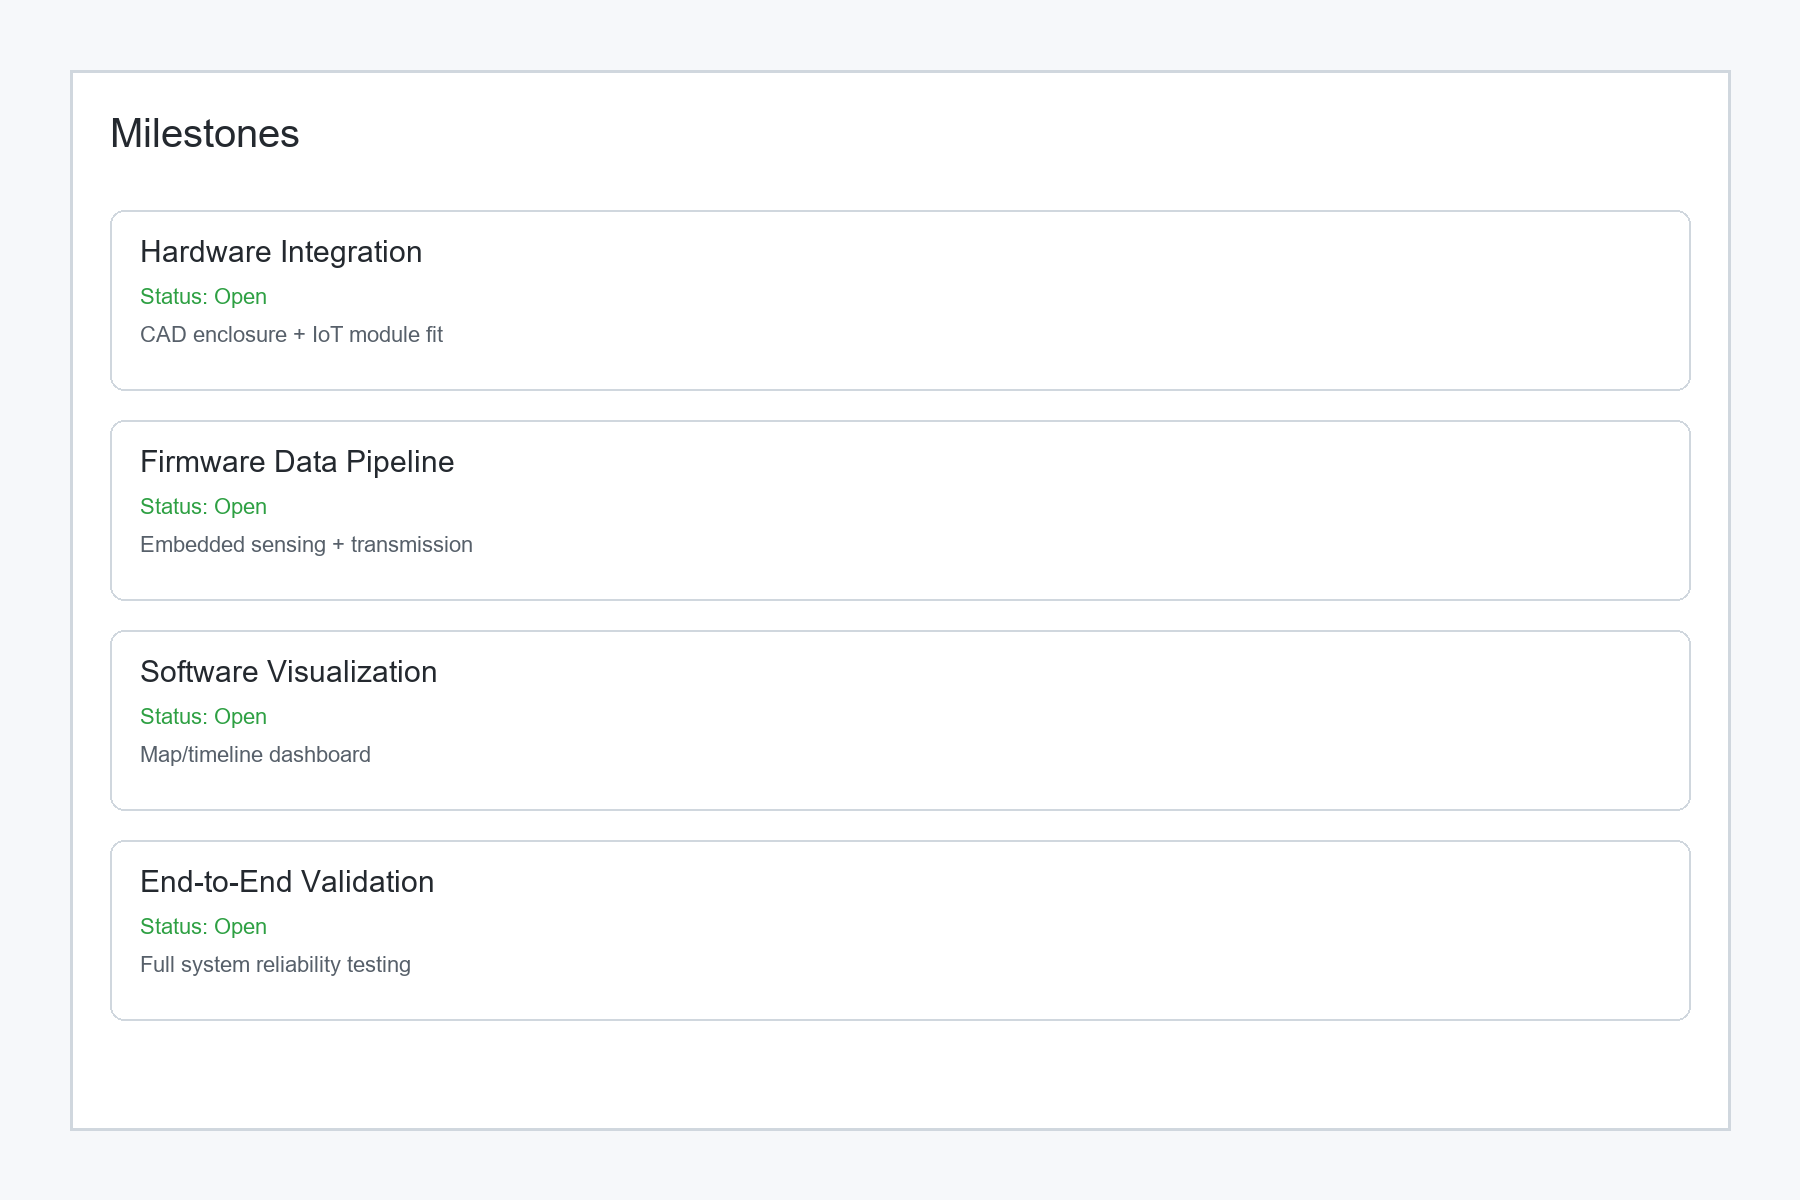
\includegraphics[width=\textwidth]{../screenshots/milestones.png}
\caption{GitHub Milestones View}
\end{figure}

\newpage
\section{Kanban Board Screenshot}
\begin{figure}[H]
\centering

\includegraphics[width=\textwidth]{../screenshots/kanban_board.png}
\caption{GitHub Kanban Board View}
\end{figure}

\end{document}
